\documentclass[11pt, oneside]{article}   	% use "amsart" instead of "article" for AMSLaTeX format
\usepackage[margin=1in]{geometry}         % See geometry.pdf to learn the layout options. There are lots.
\geometry{letterpaper}                   		% ... or a4paper or a5paper or ... 
%\geometry{landscape}                		% Activate for for rotated page geometry
%\usepackage[parfill]{parskip}    		% Activate to begin paragraphs with an empty line rather than an indent
\usepackage{graphicx}				% Use pdf, png, jpg, or eps� with pdflatex; use eps in DVI mode
								% TeX will automatically convert eps --> pdf in pdflatex		
\usepackage{amsmath}	
\usepackage{amssymb}
\usepackage{breqn}
\usepackage{natbib}
\usepackage{hyperref}
\usepackage{amsthm}
\usepackage{bm}
\usepackage{authblk}
\usepackage{listings}

\lstset{%
   basicstyle=\ttfamily
}

\newcommand{\RN}[1]{%
  \textup{\uppercase\expandafter{\romannumeral#1}}%
}

\newcommand{\mjfan}[1]{{\bf [By Minjie: #1]}}
\newtheorem{mydef}{Definition}
\newtheorem{myalg}{Algorithm}
\newtheorem{myprop}{Proposition}
\newtheorem{mythm}{Theorem}
\newtheorem{myass}{Assumption}

\hypersetup{
   bookmarks=true,         % show bookmarks bar?
   unicode=false,          % non-Latin characters in Acrobat�s bookmark
   pdftoolbar=true,        % show Acrobat�s toolbar?
   pdfmenubar=true,        % show Acrobat�s menu?
   pdffitwindow=false,     % window fit to page when opened
   pdfstartview={FitH},    % fits the width of the page to the window
   pdftitle={My title},    % title
   pdfauthor={Author},     % author
   pdfsubject={Subject},   % subject of the document
   pdfcreator={Creator},   % creator of the document
   pdfproducer={Producer}, % producer of the document
   pdfkeywords={keyword1} {key2} {key3}, % list of keywords
   pdfnewwindow=true,      % links in new PDF window
   colorlinks=true,       % false: boxed links; true: colored links
   linkcolor=red,          % color of internal links (change box color with linkbordercolor)
   citecolor=blue,        % color of links to bibliography
   filecolor=magenta,      % color of file links
   urlcolor=cyan           % color of external links
}

\title{\textbf{A Note on Spherical Needlets}}
\author{Minjie Fan \thanks{Address for correspondence: Minjie Fan, Ph.D. candidate, Department of Statistics, University of California, Davis, One Shields Avenue, Davis, CA 95616, U.S.A. \\Email: {\tt mjfan@ucdavis.edu}}}
\affil{Department of Statistics, University of California, Davis}
\date{draft of \today}							% Activate to display a given date or no date

\begin{document}
\maketitle
%\section{}
%\subsection{}
\section{Introduction}

\section{Spherical Harmonics}
Plainly speaking, the spherical harmonics $\{Y_{lm}, l=0,1,\cdots, m=-l,\cdots,l\}$ are a natural extension of the Fourier basis functions to the domain of the unit sphere $\mathbb{S}^2$.  For convenience, we employ $(\theta, \phi), 0\leq \theta \leq \pi, 0 \leq \phi <2\pi$, where $\theta$ is the co-latitude and $\phi$ is the longitude, as the spherical coordinate of $\bm{x}\in \mathbb{S}^2$. The spherical harmonics share two crucial characteristics as the Fourier basis functions. First, they are eigenfunctions of the following eigenvalue problem
\begin{equation}
\Delta_{\mathbb{S}^2} Y = -\lambda Y,
\end{equation}
where $\Delta_{\mathbb{S}^2}$ is the Laplace-Beltrami operator defined on $\mathbb{S}^2$, i.e.,
\begin{dmath}
\Delta_{\mathbb{S}^2}=\frac{1}{\sin \theta}\frac{\partial}{\partial \theta}(\sin \theta \frac{\partial}{\partial \theta})+\frac{1}{\sin^2 \theta}\frac{\partial^2}{\partial \phi^2}.
\end{dmath}
Besides, they constitute an orthonormal basis of the Hilbert space $L^2(\mathbb{S}^2)$. Thus, for any function $T$ in $L^2(\mathbb{S}^2)$, it can be uniquely expanded as 
\begin{dmath}
T(\bm{x})=\sum \limits_{l=0}^{\infty}\sum \limits_{m=-l}^{l} a_{lm}Y_{lm}(\bm{x}),
\end{dmath}
where 
\begin{dmath}\label{alm}
a_{lm}=\int_{\mathbb{S}^2} T(\bm{x})\overline{Y}_{lm}(\bm{x})d\bm{x}.
\end{dmath}

The spherical harmonics can be represented in terms of the associated Legendre polynomials.
\begin{mydef}\label{SH}
For any $l=0,1,\cdots, m=-l,\cdots,l$, the spherical harmonics
\begin{equation}
Y_{lm}(\theta, \phi)=\begin{cases} \sqrt{\frac{2l+1}{4\pi}\frac{(l-m)!}{(l+m)!}}P_{lm}(\cos \theta)\exp(im\phi)\quad m\geq 0 \\
(-1)^m \overline{Y}_{l-m}(\theta, \phi) \quad m<0,
\end{cases}
\end{equation}
where $P_{lm}$ represents the associated Legendre polynomial with subscripts $l$ and $m$.
\end{mydef}
The subscripts $l$ and $m$ entail the pattern of the waves along the latitude and longitude, where $m$ is the longitudinal wave number and $(l-m+1)/2$ is the latitudinal wave number.
Proposition \ref{addition} gives the addition formula for the spherical harmonics.
\begin{myprop}\label{addition}
(Addition Formula) For any $\bm{x}, \bm{y} \in \mathbb{S}^2$,
\begin{equation}
\sum_{m=-l}^{l} Y_{lm}(\bm{x}) \overline{Y}_{lm}(\bm{y})=\frac{2l+1}{4\pi}P_l(\langle \bm{x}, \bm{y} \rangle),
\end{equation}
where $\langle \cdot, \cdot \rangle$ denotes the inner product on $\mathbb{R}^3$ and $P_l$ represents the $l$th Legendre polynomial.
\end{myprop}

\section{Spherical Needlets}
The spherical harmonics are globally supported on the sphere and thus suffer from the same difficulties as the Fourier basis functions. For example, the Gibbs phenomenon may occur when a spherical function with small spatial scale features is approximated by a finite series of spherical harmonics. In this case, noticeable spurious global oscillations will be introduced and higher order of spherical harmonics are required to achieve a good approximation. 

In this paper, we shall review a new generation of spherical wavelets, called spherical needlets. \citep{Narcowich-etal06, Marinucci-etal08, baldi2009, Marinucci2011}. They are not only exactly localized on a finite number of frequencies, but also decay quasi-exponentially fast away from their global maximum.

\subsection{Construction of Spherical Needlets}
The construction of the spherical needlets is based on two main ideas, which are a discretization of the sphere by an exact quadrature formula and a Littlewood-Paley decomposition. Theorem \ref{quadrature} gives the exact quadrature formula.
\begin{mythm}\label{quadrature}
Denote $\mathcal{H}_l$ as the space spanned by $\{ Y_{lm}: m=-l,\cdots,l \}$, and let $\mathcal{K}_l=\bigoplus_{k=0}^l \mathcal{H}_k$. For any $l \in \mathbb{N}$, there exist a finite subset $\mathcal{X}_l=\{ \bm{\xi}_{lk}: k=1,\cdots, n_l  \}$ of $\mathbb{S}^2$ and positive real numbers $\{ \lambda_{lk}: k=1,\cdots, n_l \}$ such that 
\begin{equation}
\int_{\mathbb{S}^2} f(\bm{x})d\bm{x} = \sum \limits_{k=1}^{n_l} \lambda_{lk} f(\bm{\xi}_{lk}),
\end{equation}
for any $f \in \mathcal{K}_l$.
Here $\bm{\xi}_{lk}$ and $\lambda_{lk}$ are called cubature points and cubature weights, respectively.
\end{mythm}
The quadrature formula discretizes the sphere into cubature points and cubature weights, based on which, we present the definition of the spherical needlets.
\begin{mydef}
For a given frequency $j \in \mathbb{N}_0$ and the corresponding cubature points $\bm{\xi}_{jk}$ and cubature weights $\lambda_{jk}$ (which are obtained by Theorem \ref{quadrature} with $l=2 \lfloor B^{j+1} \rfloor$), the spherical needlets with frequency $j$ are defined as 
\begin{dmath}\label{needlet}
\psi_{jk}(\bm{x})=\sqrt{\lambda_{jk}} \sum \limits_{l=\lceil B^{j-1} \rceil}^{\lfloor B^{j+1} \rfloor} b\left( \frac{l}{B^j} \right) \sum \limits_{m=-l}^{l} Y_{lm}(\bm{\xi}_{jk})\overline{Y}_{lm}(\bm{x}),
=\sqrt{\lambda_{jk}} \sum \limits_{l=\lceil B^{j-1} \rceil}^{\lfloor B^{j+1} \rfloor} b\left( \frac{l}{B^j} \right) \frac{2l+1}{4\pi} P_l(\langle \bm{\xi}_{jk}, \bm{x} \rangle) \quad \mbox{(by Proposition \ref{addition})},
\end{dmath}
where $\bm{x} \in \mathbb{S}^2$, $B>1$ is a parameter and $b(\cdot)$ is a window function satisfying 
\begin{enumerate}
\item $b(\cdot)>0$ in $(1/B, B)$, and it equals zero otherwise.
\item For any $\eta \geq1$,
\begin{equation}
\sum \limits_{j=0}^{\infty} b^2 \left( \frac{\eta}{B^j} \right)=1.
\end{equation}
\item $b(\cdot)$ is $M$ times continuously differentiable for some $M=1,2,\cdots$ or $M=\infty$.
\end{enumerate}
\end{mydef}
Equation (\ref{needlet}) implies that the spherical needlets are real-valued functions. The window function $b(\cdot)$ plays the role of the Littlewood-Paley decomposition, i.e., it decomposes the frequency domain into several overlapping intervals $(B^{j-1}, B^{j+1}),  j=0,1,\cdots$.
Here $\bm{\xi}_{jk}$ represents the location (i.e., center) of $\psi_{jk}$, while $j$ determines to what extent $\psi_{jk}$ is spatially localized. The larger $j$, the finer $\psi_{jk}$. Varying the values of $\bm{\xi}_{jk}$ and $j$ has the same effect as translation and dilation in a multiresolution analysis. Thus, compared with the spherical harmonics,  the spherical needlets are more suited to represent spherical functions with sharp local peaks or valleys.
\subsection{Properties of Spherical Needlets}
Compared with other spherical wavelets, the spherical needlets possess several attractive features:
\begin{enumerate}
\item They are exactly localized in the frequency domain since the window function $b(\cdot)$ has compact support.
\item They are also localized in the spatial domain. Specifically, we have
\begin{equation}
\lvert \psi_{jk}(\bm{x})\rvert\leq \frac{c_M B^j}{(1+B^j \arccos(\langle \bm{\xi}_{jk},\bm{x} \rangle))^M} \quad \mbox{for any } \bm{x} \in \mathbb{S}^2,
\end{equation}
where $M\in \mathbb{N}$ such that $b$ is M times continuously differentiable, and $c_M$ is a constant regardless of $j$ and $k$.
\item The spherical needlets (together with the first spherical harmonic $Y_{00}=\sqrt{1/(4\pi)}$) constitute a Parseval tight frame, i.e., for any $T \in L^2(\mathbb{S}^2)$,
\begin{equation}\label{energy}
A\lVert T \rVert_2^2 \leq \sum \limits_{j,k} \lvert \langle T, \psi_{jk} \rangle \rvert^2+a_{00}^2 \leq B\lVert T \rVert_2^2,
\end{equation}
where $A=B=1$, and 
$$\langle T, \psi_{jk} \rangle=\int_{\mathbb{S}^2} T(\bm{x})\psi_{jk}(\bm{x})d\bm{x},$$ 
which are called needlet coefficients and denoted as $\beta_{jk}$,
\begin{dmath}\label{needlet_coef}
\beta_{jk}=\int_{\mathbb{S}^2} T(\bm{x})\psi_{jk}(\bm{x})d\bm{x}
=\sqrt{\lambda_{jk}}\sum \limits_{l=0}^{\infty} b\left( \frac{l}{B^j} \right) \sum \limits_{m=-l}^{l} a_{lm} Y_{lm}(\bm{\xi}_{jk})
=\sqrt{\lambda_{jk}}\sum \limits_{l=\lceil B^{j-1} \rceil}^{\lfloor B^{j+1} \rfloor} b\left( \frac{l}{B^j} \right) \sum \limits_{m=-l}^{l} a_{lm} Y_{lm}(\bm{\xi}_{jk}),
\end{dmath}
where $a_{lm}$ has been defined by equation (\ref{alm}).

Equation (\ref{energy}) entails that (1) the needlet expansion preserves the ``energy" of the function in the sense of L2-norm; (2) the dual frame coincides with the frame itself, and thus the spherical needlets have the perfect reconstruction property of orthonormal bases, i.e.,
\begin{equation}\label{reconstruction}
T(\bm{x})=a_{00}Y_{00}(\bm{x})+\sum \limits_{j,k} \beta_{jk}\psi_{jk}(\bm{x}).
\end{equation}
\item The spherical needlets are almost orthogonal, i.e., if  $\lvert j-j' \rvert \geq 2$,
$$\langle \psi_{jk}, \psi_{j'k'} \rangle=\int_{\mathbb{S}^2}\psi_{jk}(\bm{x}) \psi_{j'k'}(\bm{x}) d\bm{x} = 0.$$
\item The spherical needlets $\psi_{jk}$ and $\psi_{jk'}$ are asymptotically uncorrelated as the frequency increases and the distance between them is fixed, i.e.,
$$\left\lvert \frac{\langle \psi_{jk}, \psi_{jk'} \rangle}{\lVert \psi_{jk} \rVert \lVert \psi_{jk'} \rVert} \right\rvert \leq \frac{C_M}{(1+B^j \arccos(\langle \bm{\xi}_{jk},\bm{\xi}_{jk'} \rangle))^M},$$
where
$$\langle \psi_{jk}, \psi_{jk'} \rangle = \sqrt{\lambda_{jk} \lambda_{jk'}}\sum_l b^2\left(\frac{l}{B^j}\right)\frac{2l+1}{4\pi}P_l( \langle \bm{\xi}_{jk}, \bm{\xi}_{jk'} \rangle).$$
The proof is omitted here, and we refer to Lemma 3 in \citet{baldi2009}.
\end{enumerate}

\subsection{Implementation}
The needlet coefficients can be obtained by equation (\ref{needlet_coef}), which involves the spherical harmonic coefficients. When the sampling locations are on an equiangular grid, we can use the package  S2Kit \citep{Healy-etal03, Kostelec-etal04} to perform a fast spherical harmonic transform. When the observations are irregularly spaced, the spherical harmonic coefficients can be estimated empirically by
\begin{equation}\label{alm_irr}
\widehat{a}_{lm}=\sum \limits_{i=1}^{N}w_i T(\bm{x}_i) \overline{Y}_{lm}(\bm{x}_i),
\end{equation}
where $\bm{x}_i$ are the sampling locations, and each $w_i$ is an appropriate cubature weight based on the surface area associated with $\bm{x}_i$. For example, each $w_i$ can be estimated to be the area of the corresponding spherical polygon determined by the Voronoi diagram of all the sampling locations.

The cubature points $\bm{\xi}_{jk}$ and cubature weights $\lambda_{jk}$ are assumed to be provided by the HEALPix discretization of the sphere \citep{Gorski-etal05}. Plainly speaking, the HEALPix grid discretizes the sphere into $N_{\rm pix}$ pixels with equal area, where $N_{\rm pix}=12N_{\rm side}^2$ and $N_{\rm side}$ is required to be a power of two that measures the resolution of the discretization. We specify the cubature points $\bm{\xi}_{jk}$ as the center of each pixel, and 
the cubature weights as the area of each pixel, i.e.,
\begin{equation}
\lambda_{jk}=\frac{4\pi}{N_{\rm pix}}.
\end{equation}

Suppose the highest frequency of the spherical harmonics that can be reliably extracted from the observations is $l_{\max}$. The maximum index $j_{\max}$ of the spherical needlets is the maximal $j$ such that $\lceil B^{j-1} \rceil \leq l_{\max}$. For each $j$ between $0$ and $j_{\max}$, the value of $N_{\rm side}$ is determined by the inequality $\lfloor B^{j+1} \rfloor \leq 2N_{\rm side}$ such that the quadrature formula in Theorem \ref{quadrature} holds approximately \citep{Pietrobon-etal10}. There are other ways of discretizating the sphere with an exact quadrature formula and (almost) equal cubature weights, such as GLESP\citep{Doroshkevich2005} and (symmetric) spherical t-designs \citep{Womersley-15}.

Computing the needlet coefficients by equation (\ref{needlet_coef}) is equivalent to performing an inverse spherical harmonic transform. The latter can be done in an efficient way by utilizing the distinct structure of the HEALPix grid. Specifically, the cubature points are arranged in a number of iso-latitude rings. The points on each ring share the same value of the co-latitude. Thus, the associated Legendre polynomials in the definition of the spherical harmonics only need to be evaluated once for all the points on each ring. Moreover, the grid is symmetric with respect to the equator, which reduces the computational cost for evaluating the associated Legendre polynomials by half. The inverse fast Fourier transform is also implemented to further reduce the computational cost. The Appendix gives the details of the implementation. Note that the time complexity of computing the needlet coefficients is $\mathcal{O}(l_{\max}^3)$. Other computational techniques, such as parallelization and butterfly matrix compression are discussed in \citep{Hupca-etal12, Seljebotn-2012}.

\section{NeedMat: A Matlab Package for Spherical Needlets}
Currently, there are several packages available for spherical needlets, such as Needatool \citep{Pietrobon-etal10} and S2LET \citep{Leistedt-2013}. The former is written in Fortran and the latter is not easy to install because of the dependencies. In this section, we shall introduce a Matlab package for spherical needlets, called \textbf{NeedMat}, which is easy to install and use. In the package, the window function $b(\cdot)$ is constructed according to \citet{Marinucci-etal08}.
\subsection{Plot of Spherical Needlets}
The spherical needlet $\psi_{jk}$ can be plotted by the function {\tt plot\_needlets(B, j, k, res)}, where
the argument {\tt res} is a parameter controlling the resolution of the plots.
Figures \ref{plot1}-\ref{plot2} show the plots of the spherical needlet with $j=3$ and $k=100$.

\begin{figure}[htbp] %  figure placement: here, top, bottom, or page
   \centering
   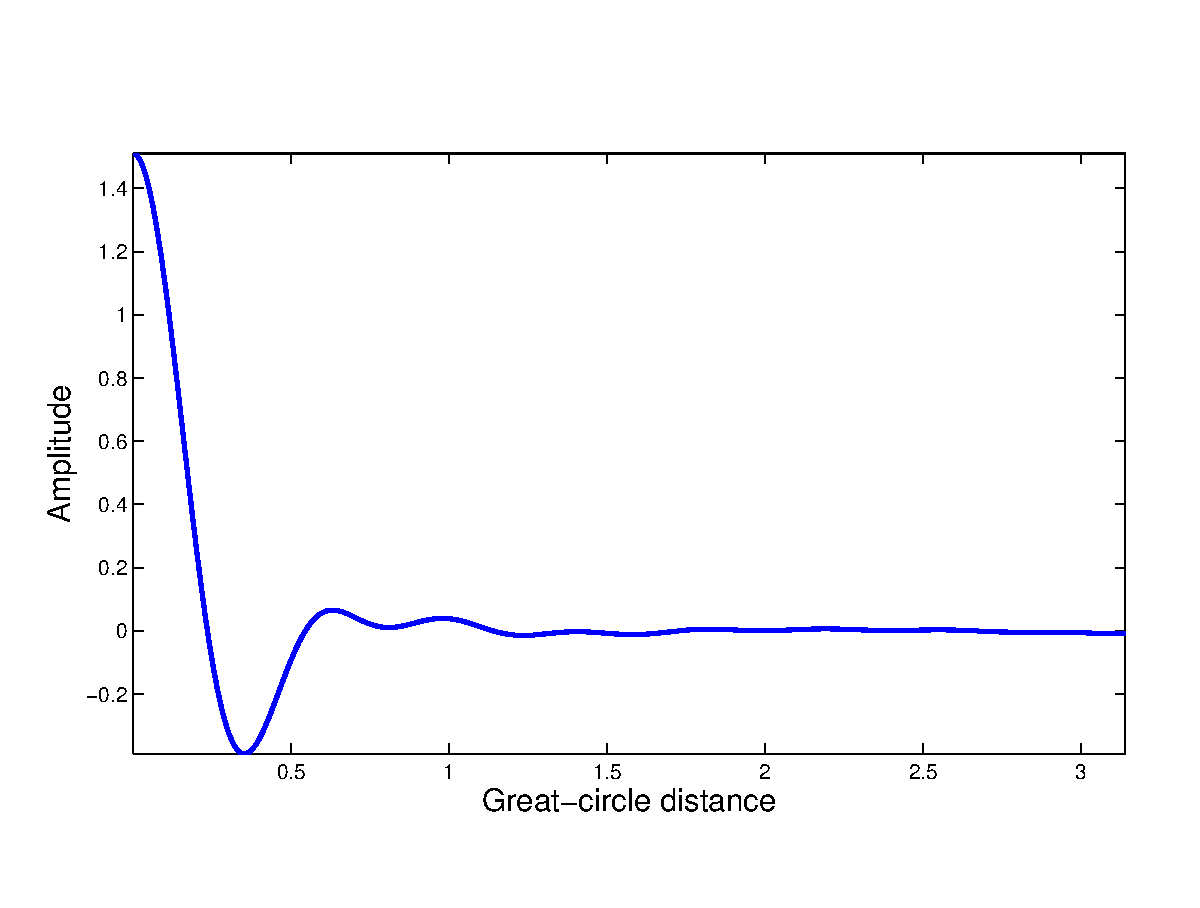
\includegraphics[width=4in]{plot.eps} 
   \caption{Plot of the spherical needlet $\psi_{jk}$ with $j=3$ and $k=100$ as a function of the great-circle distance between $\bm{\xi}_{jk}$ and $\bm{x}$. Note that this plot remains the same for an arbitrary value of $k$.}
   \label{plot1}
\end{figure}
\begin{figure}[htbp] %  figure placement: here, top, bottom, or page
   \centering
   \includegraphics[width=3.5in]{plot2.eps} 
   \caption{Plot of the spherical needlet $\psi_{jk}$ with $j=3$ and $k=100$ on the sphere. The sphere has been projected to an ellipse by the Hammer projection.}
   \label{plot2}
\end{figure}

\subsection{Example: Approximation of a Wendland Radial Basis Function}
In this subsection, we present a short example to demonstrate the usage of NeedMat and the superiority of the spherical needlets to the spherical harmonics in capturing small spatial scale features. The function to be approximated is
$$\varphi(\bm{x})=\varphi_0\left(\arccos \langle \bm{\xi}_0, \bm{x} \rangle/\rho\right),$$
where $\bm{\xi}_0$ is the center of the function, $\rho$ is a spatial scale parameter, and $\varphi_0(\cdot)$ is the Wendland radial basis function \citep{Wendland-1995} in $C^4$
$$\varphi_0(d) = 
\begin{cases}
(1-d)^6(35d^2+18d+3)/3 & \mbox{for } 0\leq d \leq 1\\
0 & \mbox{otherwise}
\end{cases}.
$$
\begin{figure}[htbp] %  figure placement: here, top, bottom, or page
   \centering
   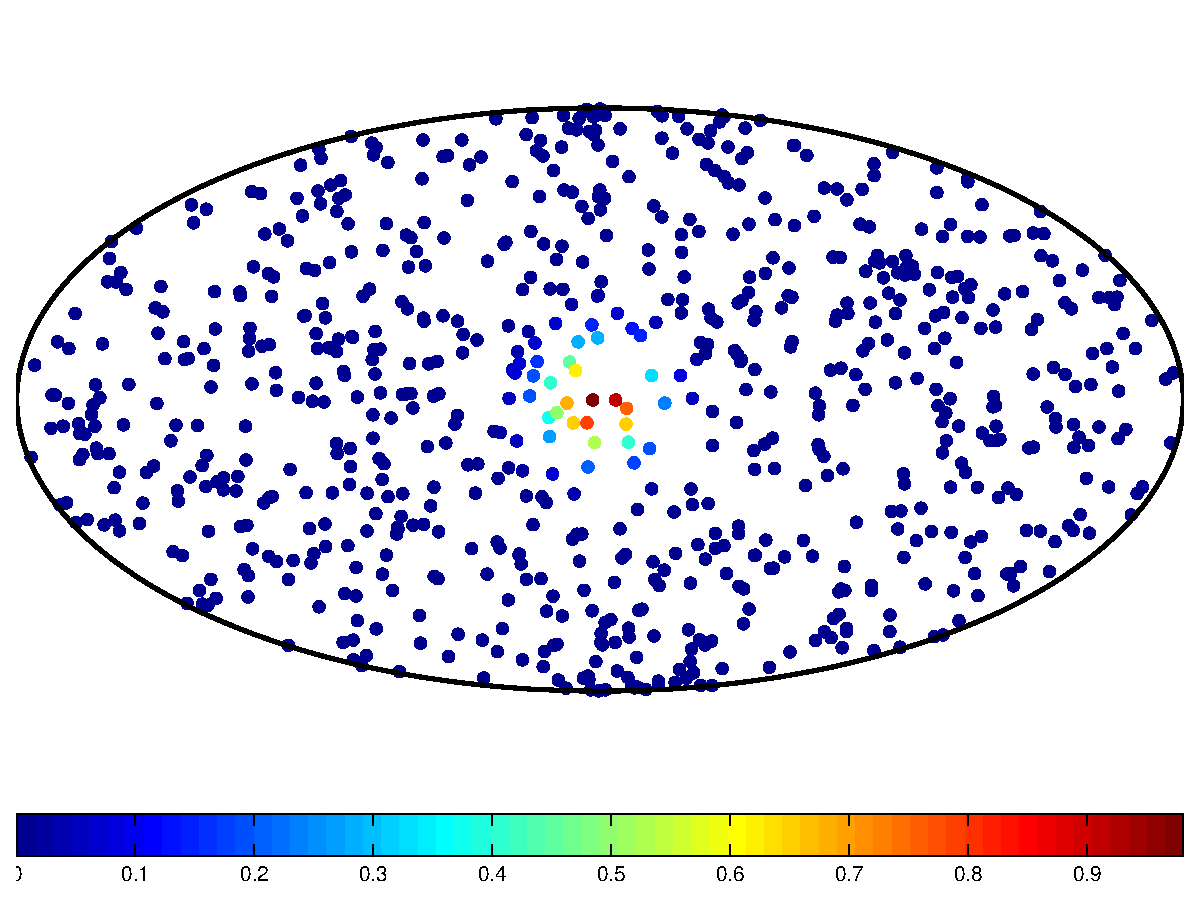
\includegraphics[width=3.5in]{wendland.eps} 
   \caption{Observations of the Wendland radial basis function in $C^4$ on a perturbed HEALPix grid with $768$ grid points.}
   \label{wendland}
\end{figure}
We specify $\bm{\xi}=(\pi/2, \pi)$ in spherical coordinates and $\rho=\pi/4$. The observations are on a perturbed HEALPix grid with $768$ grid points, as shown in Figure \ref{wendland}.  The spherical harmonic coefficients are estimated by equation (\ref{alm_irr}) with $w_i$ being determined by the Voronoi diagram
\begin{lstlisting}
alm = spharmonic_tran_irr(theta, phi, f_wend, l_max);
\end{lstlisting}
\begin{figure}[htbp] %  figure placement: here, top, bottom, or page
   \centering
   \includegraphics[width=3.5in]{fit1.eps} 
   \caption{example caption}
   \label{fig:example}
\end{figure}

\begin{figure}[htbp] %  figure placement: here, top, bottom, or page
   \centering
   \includegraphics[width=3.5in]{fit2.eps} 
   \caption{example caption}
   \label{fig:example}
\end{figure}
\section{Conclusion}
\section*{Acknowledgement}
This research is partially supported by NSF grants AGS-1025089, PLR-1443703 and DMS-1407530. I am grateful to my advisors, Thomas C.M, Lee, Debashis Paul and Tomoko Matuo, for their kindness, guidance, and encouragement.

\section*{Appendix: Fast Inverse Spherical Harmonic Transform}
We are interested in the following inverse spherical harmonic transform
$$\sum \limits_{l=l_{\rm st}}^{l_{\rm en}}\sum \limits_{m=-l}^l a_{lm} Y_{lm}(\bm{\xi}_{jk}),$$
where $\bm{\xi}_{jk}$ is one of the points on the HEALPix grid. Suppose $\bm{\xi}_{jk}$ is the $p$-th point ($0\leq p \leq n_r-1$) on the $r$-th ring ($1\leq r \leq N_{\rm ring}$). In spherical coordinates, 
$\bm{\xi}_{jk}=(\theta_r, \phi_{rp})$, where $\phi_{rp}=\phi_{r0}+2\pi p/n_r$.
Using the fact that $a_{l-m}=(-1)^m \overline{a}_{lm}$ and $Y_{l-m}=(-1)^m \overline{Y}_{lm}$, we have
$$
\sum \limits_{l=l_{\rm st}}^{l_{\rm en}}\sum \limits_{m=-l}^l a_{lm} Y_{lm}(\bm{\xi}_{jk})
=\RN{1}+\RN{2}+\overline{\RN{2}}, 
$$
where 
$$\RN{1}=\sum \limits_{l=l_{\rm st}}^{l_{\rm en}} a_{l0}Y_{l0} (\bm{\xi}_{jk}),$$
and
$$\RN{2}=\sum \limits_{l=l_{\rm st}}^{l_{\rm en}}\sum \limits_{m=1}^l a_{lm} Y_{lm}(\bm{\xi}_{jk}).$$
Define $\widetilde{P}_{lm}$ as the normalized associated Legendre polynomial with subscripts $l$ and $m$,
$$\widetilde{P}_{lm}(x)=\sqrt{\frac{2l+1}{4\pi}\frac{(l-m)!}{(l+m)!}}P_{lm}(x).$$
Then
$$\RN{1}=\sum \limits_{l=l_{\rm st}}^{l_{\rm en}} a_{l0} \widetilde{P}_{l0}(\cos \theta_r),$$
and
$$\RN{2}=\sum \limits_{l=l_{\rm st}}^{l_{\rm en}} \sum \limits_{m=1}^l a_{lm} \widetilde{P}_{lm}(\cos \theta_r) \exp(im \phi_{rp}).$$
Interchanging the order of summation in $\RN{2}$, we have
\begin{dmath*}
\RN{2}=\sum \limits_{m=1}^{l_{\rm en}} \left[\sum \limits_{l= \max \{ m, l_{\rm st} \}}^{l_{\rm en}}a_{lm} \widetilde{P}_{lm}(\cos \theta_r)\right] \exp(im \phi_{rp})=\sum \limits_{m=1}^{l_{\rm en}} q_{mr}  \exp(im \phi_{rp}).
\end{dmath*}
Let $m=n_rs+t$. Then
\begin{dmath*}
\RN{2}=\sum \limits_{t=0}^{n_r-1} \left\{ \sum_s q_{n_rs+t, r} \exp \left[i(n_rs+t)\phi_{r0}\right] \right\}w^{-pt}
=\sum \limits_{t=0}^{n_r-1} \tau_{tr} w^{-pt},
\end{dmath*}
where $w=\exp (-2\pi i/n_r)$.
Thus, $\RN{2}$ can be obtained by the inverse fast Fourier transform.
\bibliography{references}
\bibliographystyle{rss}

\end{document}  